% Shared TikZ diagrams for LocalMesh Phase 1
\usepackage{tikz}
\usetikzlibrary{arrows.meta,calc,fit,positioning,shapes.geometric}

\definecolor{lmNavy}{HTML}{1B3A4B}
\definecolor{lmTeal}{HTML}{2A9D8F}
\definecolor{lmSand}{HTML}{E9C46A}
\definecolor{lmCoral}{HTML}{E76F51}
\definecolor{lmInk}{HTML}{264653}
\definecolor{lmMist}{HTML}{F4F1DE}
\definecolor{lmBlue}{HTML}{3D5A80}

\newcommand{\lmbox}[3]{%
  \node[draw=#1, fill=#1!12, line width=0.8pt, rounded corners=3pt,
        align=center, font=\scriptsize\sffamily, inner sep=5pt, #3] {#2};
}

\newcommand{\figcaptionstyle}{\captionsetup{font=small,labelfont={bf,sf},textfont=it}}

% ---------- Figure: LAN topology ----------
% Backends live INSIDE Your Mac (UTM). HTTPS is client -> Manohar first.
% The dashed arrow is DNS only (A-record), not the data path.
\newcommand{\drawTopology}{%
\begin{tikzpicture}[
  font=\sffamily\scriptsize,
  box/.style={draw=##1, fill=##1!10, line width=0.85pt, rounded corners=3pt,
              align=center, inner sep=5pt, minimum width=2.85cm, minimum height=1.25cm},
  lan/.style={draw=lmNavy, fill=lmNavy!6, rounded corners=6pt},
]
  \node[lan, minimum width=16.0cm, minimum height=7.35cm] (lan) at (0.15,0.05) {};
  \node[font=\sffamily\bfseries\small, text=lmNavy] at (0.15,3.25) {Private Wi-Fi / LAN  (two Macs + clients only)};

  \node[draw=lmNavy, fill=lmNavy!14, rounded corners=5pt, minimum width=7.5cm, minimum height=4.15cm] (host) at (-3.55,-0.45) {};
  \node[font=\sffamily\bfseries\scriptsize, text=lmNavy, anchor=north] at (-3.55,1.5) {Your Mac --- 10.7.12.104  (one Wi-Fi host)};

  \node[box=lmNavy] (dns) at (-3.55,0.55) {dnsmasq UDP/53\\answers \texttt{app.localmesh.test}};
  \node[box=lmBlue] (a) at (-5.15,-1.35) {\textbf{UTM guest A}\\not on Wi-Fi\\:3001 inside host};
  \node[box=lmCoral] (b) at (-1.95,-1.35) {\textbf{UTM guest B}\\not on Wi-Fi\\:3002 inside host};

  \node[box=lmTeal] (edge) at (4.55,1.05) {\textbf{Manohar's Mac}\\10.7.2.38\\nginx :8443};
  \node[box=lmSand, text=lmInk] (cli) at (4.55,-1.55) {\textbf{LAN client}\\browser / curl\\name, never backend IP};

  \draw[-{Latex}, lmNavy, densely dashed, thick] (dns.east) -- node[above, font=\tiny, align=center] {DNS A-record only\\not HTTPS} (edge.west);
  \draw[-{Latex}, lmTeal, very thick] (cli) -- node[right, font=\tiny] {1. HTTPS :8443} (edge);
  \draw[-{Latex}, lmBlue, thick] (edge.south west) -- node[below, font=\tiny, sloped, pos=0.45] {2. proxy 10.7.12.104:3001/3002} (host.east);
\end{tikzpicture}%
}

% ---------- Figure: request path ----------
\newcommand{\drawRequestPath}{%
\begin{tikzpicture}[font=\sffamily\tiny, node distance=0.35cm and 0.28cm]
  \tikzset{s/.style={draw=##1, fill=##1!14, rounded corners=2pt, align=center,
           inner sep=4pt, minimum height=1.05cm, minimum width=2.15cm, line width=0.7pt}}
  \node[s=lmNavy] (1) {1. DNS query\\UDP/53\\10.7.12.104};
  \node[s=lmTeal, right=of 1] (2) {2. A record\\app.localmesh.test\\$\to$ 10.7.2.38};
  \node[s=lmBlue, right=of 2] (3) {3. TCP\\SYN / SYN-ACK / ACK\\:8443};
  \node[s=lmSand, right=of 3] (4) {4. TLS 1.3\\team CA\\app cert};
  \node[s=lmCoral, right=of 4] (5) {5. HTTP/2\\nginx $\to$\\10.7.12.104:3001/2};
  \foreach \a/\b in {1/2,2/3,3/4,4/5}
    \draw[-{Latex}, thick, lmInk] (\a) -- (\b);
\end{tikzpicture}%
}

% ---------- Figure: UTM forwards ----------
\newcommand{\drawUtm}{%
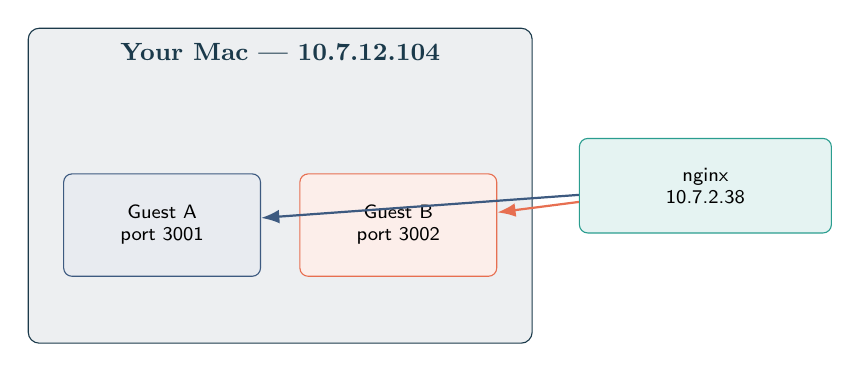
\begin{tikzpicture}[font=\sffamily\scriptsize]
  \node[draw=lmNavy, fill=lmNavy!8, rounded corners=4pt, minimum width=6.4cm, minimum height=4.0cm] (host) at (0,0) {};
  \node[font=\bfseries\small, text=lmNavy] at (0,1.7) {Your Mac --- 10.7.12.104};
  \node[draw=lmBlue, fill=lmBlue!12, rounded corners=3pt, align=center, minimum width=2.5cm, minimum height=1.3cm] (va) at (-1.5,-0.5) {Guest A\\port 3001};
  \node[draw=lmCoral, fill=lmCoral!12, rounded corners=3pt, align=center, minimum width=2.5cm, minimum height=1.3cm] (vb) at (1.5,-0.5) {Guest B\\port 3002};
  \node[draw=lmTeal, fill=lmTeal!12, rounded corners=3pt, align=center, minimum width=3.2cm, minimum height=1.2cm] (ng) at (5.4,0) {nginx\\10.7.2.38};
  \draw[-Latex, thick, lmBlue] (ng) -- (va);
  \draw[-Latex, thick, lmCoral] (ng) -- (vb);
\end{tikzpicture}%
}

% ---------- Figure: TLS chain ----------
\newcommand{\drawTls}{%
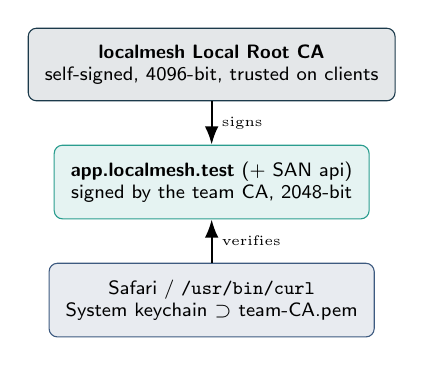
\begin{tikzpicture}[font=\sffamily\scriptsize, node distance=0.55cm]
  \node[draw=lmNavy, fill=lmNavy!12, rounded corners=3pt, align=center, inner sep=6pt] (ca)
    {\textbf{localmesh Local Root CA}\\self-signed, 4096-bit, trusted on clients};
  \node[draw=lmTeal, fill=lmTeal!12, rounded corners=3pt, align=center, inner sep=6pt, below=of ca] (srv)
    {\textbf{app.localmesh.test} (+ SAN api)\\signed by the team CA, 2048-bit};
  \node[draw=lmBlue, fill=lmBlue!12, rounded corners=3pt, align=center, inner sep=6pt, below=of srv] (cli)
    {Safari / \texttt{/usr/bin/curl}\\System keychain $\supset$ team-CA.pem};
  \draw[-{Latex}, thick] (ca) -- node[right, font=\tiny] {signs} (srv);
  \draw[-{Latex}, thick] (cli) -- node[right, font=\tiny] {verifies} (srv);
\end{tikzpicture}%
}

% ---------- Figure: OSI mapping ----------
\newcommand{\drawOsi}{%
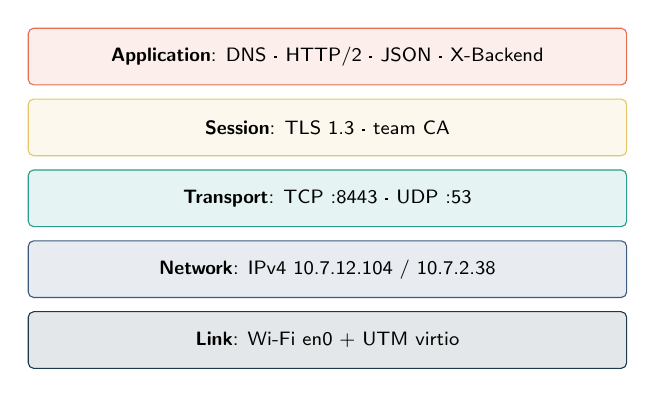
\begin{tikzpicture}[font=\sffamily\scriptsize]
  \foreach \y/\c/\t/\n in {
    4.2/lmCoral/Application/{DNS · HTTP/2 · JSON · X-Backend},
    3.3/lmSand/Session/{TLS 1.3 · team CA},
    2.4/lmTeal/Transport/{TCP :8443 · UDP :53},
    1.5/lmBlue/Network/{IPv4 10.7.12.104 / 10.7.2.38},
    0.6/lmNavy/Link/{Wi-Fi en0 + UTM virtio}
  } {
    \node[draw=\c, fill=\c!12, rounded corners=2pt, minimum width=7.6cm,
          minimum height=0.72cm, anchor=west] at (0,\y) {\textbf{\t}: \n};
  }
\end{tikzpicture}%
}
